

\documentclass[tikz,border=5mm]{standalone}
\usetikzlibrary{arrows,calc}
\begin{document}
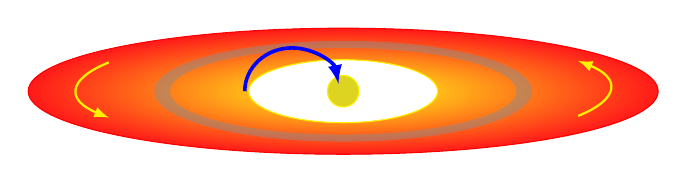
\begin{tikzpicture}
% \node(x0)  at (-0.33,0.1) {\includegraphics[height=8cm,width=12cm,angle=0,trim={3cm 2.5cm 3.5cm 2cm},clip]{../figs/ctts2.pdf}};

\def\incurve{(0,0) ellipse (1.2 and 0.4)}
\def\outcurve{(0,0) ellipse (4 and 0.8)}

\def\ringin{(0,0) ellipse (2.2 and 0.55)}
\def\ringout{(0,0) ellipse (2.4 and 0.64)}

% \def\incurve{(0,0) ellipse (1.2 and 0.4)}
% \def\outcurve{(0,0) ellipse (4 and 0.8)}


\fill[inner color=yellow!90, outer color=red!90,even odd rule] \incurve \outcurve;
\fill[color=gray!90,even odd rule, opacity=0.5] \ringin \ringout;

\draw[yellow] \incurve; 
\draw[red] \outcurve;
% \draw[->,>=stealth',semithick] (-5:3) arc[radius=0.3, start angle=-60, end angle=60];
 \draw[thick, yellow, -latex] (-6:3) arc   (-30:30:3cm and 0.7cm);
 \draw[thick, yellow, -latex] (173:3) arc   (150:210:3cm and 0.7cm);

\draw [yellow, fill=yellow!85!black] (0,0) circle (0.2);
%  \draw[thick, blue, -latex] (150:0.2) arc (10:350:0.5cm and 0.6cm);
 \draw[thick, blue, -latex, line width=1.3pt] (-1.25,0) arc (180:10:0.6cm and 0.55cm);

 



\end{tikzpicture}
\end{document}
